\clearpage
\chapter{Results and analysis}\label{ch:results}
\begingroup
\clubpenalty=10000
\makeatletter\@clubpenalty=10000\makeatother
\widowpenalty=10000
\brokenpenalty=10000

We first ask whether the state retains useful current anatomy, then whether earlier MRI improves prediction beyond that state. Anatomical supervision, additional sequences and higher-resolution features improve several current-state readouts. Forecasting gains are narrower, and the matched comparisons do not establish a consistent, practically useful contribution from history. The acquisition results test one further use of the state: choosing another sequence. Results are documented in the project research record \cite{record}. Unless stated otherwise, scores average observations within each patient and then give patients equal weight.

\section{Current anatomy and observed change}

Mask supervision gives the encoder information about where tissue is, alongside the volume target. The densely supervised spatial pipeline reduces LUMIERE current-volume MAE from 1.500 to 1.115 log1p(mm³) over 149 visits from 26 patients. Its spatial encoder receives mask and volume supervision, while the fixed-encoder control receives scalar-volume supervision. The gain is in-domain: on SAILOR, the spatial model scores 2.240 against 2.111 for a source-fitted constant predictor, with a paired interval spanning zero.

Matching the architecture, supervision and training draws isolates the effect of pretrained initialization. BrainIAC initialization improves nonempty-compartment Dice from 0.158 to 0.198 over 60 visits from 13 reused LUMIERE patients. The paired gain is 0.040, with an adjusted 97.5\% interval of [0.020, 0.059], and both seeds favor pretraining. Volume error remains within the allowed +0.05 log1p(mm³) retention margin. Pretraining helps overlap under this comparison, although Dice remains low in both models.

A readout can also recover change between two available scans. The trained nonlinear change head reduces LUMIERE signed-occupancy MAE from 0.48351 to 0.27041 under matched supervision. The frozen local-occupancy contrast is -0.00307, with an adjusted interval of [-0.00800, +0.00264]. Because both scans are observed, the stronger trained readout establishes recovery of observed change; it does not yet test prediction of a future scan.

\section{Accounting for postoperative cavity}

For postoperative anatomy, treating cavity as a separate category reduces its confusion with core. The matched comparison uses 106 MU visits from 32 selection patients and 178 LUMIERE visits from 18 selection patients. Both checkpoints are scored against the same reference masks over the full annotated volume, including labeled tissue outside the MRI foreground.

On MU, original-three-compartment Dice rose from 0.62942 to 0.66392. Core absolute volume error fell from 8.043 to 1.666 mL, and predicted core inside reference cavity fell from 6.143 to 0.784 mL. Figure~\ref{fig:cavity} shows the paired effects. New cavity Dice was 0.55783 on 97 nonempty visits from 30 patients, with a 95\% patient-bootstrap interval of [0.47428, 0.63803]. On nine cavity-empty visits from five patients, false-positive cavity averaged 4.112 mL.

\begin{figure}[htbp]\centering
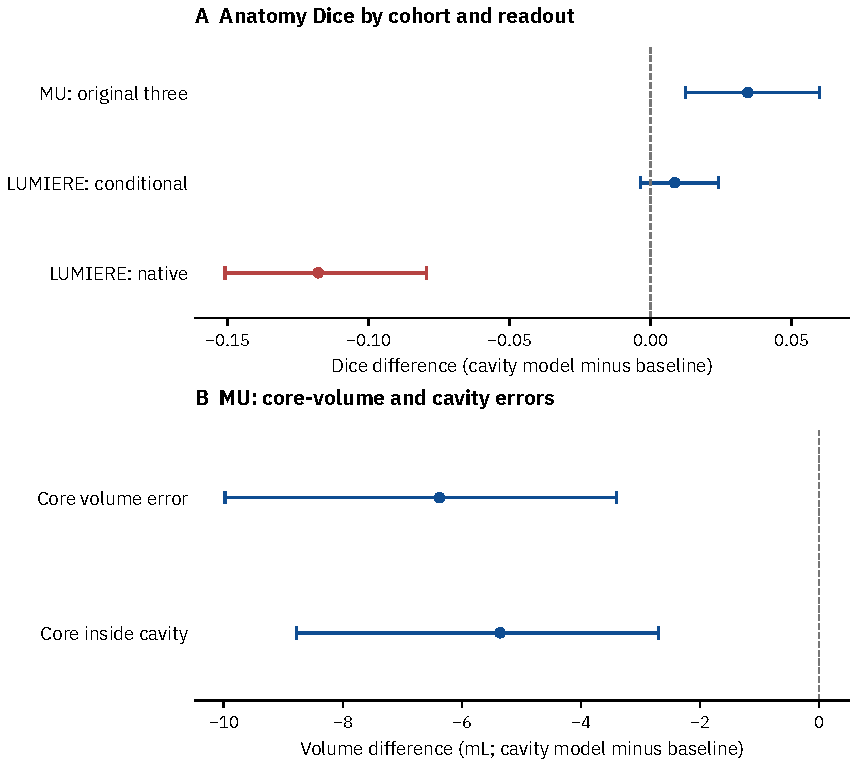
\includegraphics[width=\linewidth]{figures/updated_cavity.pdf}
\caption[Cavity supervision and readout effects]{Cavity-model changes relative to the preserved observation baseline. Panel A scores the original three lesion compartments: positive Dice differences favor the cavity model. Conditional LUMIERE scoring removes the cavity logit; native scoring keeps it. Panel B shows MU volume changes, where negative values favor the cavity model. Bars are unadjusted 95\% paired patient-bootstrap intervals from 4,000 draws. MU has 106 visits from 32 patients; LUMIERE has 178 visits from 18. All are reused selection data.}\label{fig:cavity}
\end{figure}

On LUMIERE, conditional four-category lesion Dice changed from 0.71045 to 0.71904, while the native five-category output scored 0.59256. The latter difference was -0.11789 [-0.15097, -0.07964]. LUMIERE has no cavity references; the native score measures agreement with its available labels. Missing-FLAIR lesion MAE increased from 0.57373 to 0.59040, a paired difference of +0.01667 [0.00458, 0.02658]. The MU improvement therefore comes with a cross-dataset and cross-task tradeoff: the native LUMIERE readout agrees less well with its available anatomical labels, and missing-FLAIR error rises.

\section{Completing missing MRI}

Completing current FLAIR tests information that the available sequences and their representation retain about an unobserved image. We compare CT1 alone, CT1 plus T1, and CT1 plus T1 plus T2 using three matched seeds and 116 visits from 18 LUMIERE patients; 112 visits contribute lesion scores. Lesion MAE fell from 0.90614 to 0.85781 after adding T1, then to 0.59294 after adding T2. The respective reductions were 5.33\% and 30.88\%. All four primary intervals, covering lesion and whole-brain error for both additions, favored the added sequence after multiplicity adjustment. T2 improved both endpoints in every scoring patient after seed averaging.

The decoder also needs access to useful spatial detail. A separate comparison enables or zeros its higher-resolution feature path. Enabling that path reduced lesion MAE from 0.75641 to 0.63469 and lesion-band gradient error from 0.23161 to 0.20923. All three seeds favored spatial access on lesion, gradient and nonlesion error. The paired lesion reduction was 0.12172 [0.08854, 0.14897], or 16.09\% of the zeroed arm's error. The direct-image sequence-addition reference scores 0.59294 on the same lesion endpoint. The 16.09\% reduction belongs to the spatial-path comparison; it is not a further reduction from the sequence-addition model. Figure~\ref{fig:completion} keeps these two comparisons separate.

\begin{figure}[htbp]\centering
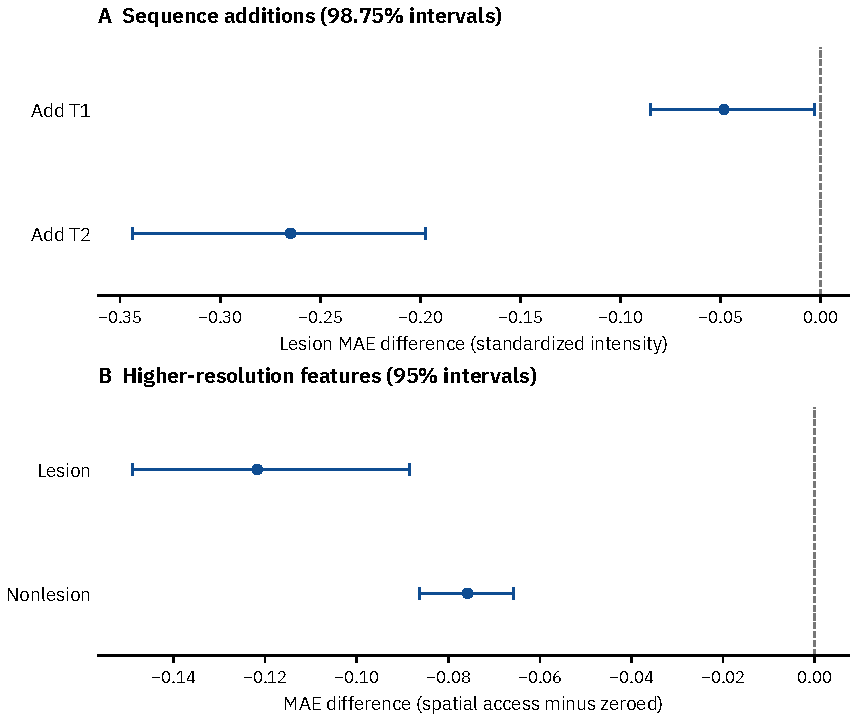
\includegraphics[width=\linewidth]{figures/updated_completion.pdf}
\caption[Sequence additions and spatial access]{FLAIR completion on reused LUMIERE development patients. Negative differences favor the added input or enabled spatial path. Panel A shows adjusted 98.75\% paired patient-bootstrap intervals from the sequence-addition study; panel B shows 95\% intervals from the spatial-feature study. Each comparison averages three seed scores over 18 patients. Lesion scoring uses 112 visits; nonlesion scoring uses 116. The two panels have independent scales.}\label{fig:completion}
\end{figure}

The compact state does not preserve all of the full predictor's completion performance. With new readouts fitted to frozen compact states, lesion MAE was 1.01734 for the enabled encoder's compact state and 0.74812 for the zeroed encoder's state; the full spatial-feature predictor scored 0.63469. The frozen-state segmentation study then reused the full learned state for segmentation on 116 visits from 18 patients, averaging three seeds. Its frozen learned features improved Dice over frozen random features by 0.06679 [0.05128, 0.08271]. Direct-image adaptation scored 0.07915 higher than the frozen learned state, with a paired 95\% difference interval of [0.06587, 0.09343]. That deficit exceeded the allowed 0.05 margin. The full representation occupies 334.75 MiB per visit, 4.05 times the Float32 input payload. Its learned features are useful, but retaining them has a substantial storage cost and still leaves a gap to direct-image adaptation.

\section{Forecasting anatomical measurements}\label{sec:initial-results}

Forecasting depends on both the current anatomical estimate and the prediction of its change. In the representation-forecast comparison, current-scan, mean-history and JEPA next-visit volume-error ratios relative to measured persistence were 1.325, 1.377 and 1.393 on LUMIERE. On SAILOR they were 3.374, 5.235 and 2.883. MRI models estimate anatomy from images, whereas persistence receives current mask measurements. These ratios therefore include the cost of estimating the current state. The matched history comparisons below test the additional value of earlier visits.

The frozen-history study compared history with latest-only MRI using the same past timing and availability information. On 75 pairs from 18 LUMIERE patients, history minus latest-only CRPS was +0.003 log1p(mm³), with an adjusted 99\% interval of [-0.047, +0.052]. The joint-training study allowed forecast gradients into the encoder; current-state MAE rose from 1.473 to 1.540 in the history arm. The supplied-horizon study provided the realized follow-up interval and obtained a 0.05\% history CRPS reduction, below its fixed 5\% criterion.

Adding recorded treatment status to MRI history gives a further test of the available context, using 242 SAILOR pairs from 27 patients. The CRPS difference was +0.001 [-0.081, +0.082], using a 99\% patient-bootstrap interval. The input was a coarse per-session status category whose prospective availability was unverified.

Supplying measured current anatomy removes the encoder's estimation error from the numerical forecast. With the retrospective interval also supplied, current-only CRPS was 1.007 against persistence at 1.120 on 253 pairs from 48 LUMIERE patients. The paired difference was -0.113 [-0.196, -0.031], using an adjusted 97.5\% interval. History reduced the point score by another 2.21\%, with an interval spanning zero. Transferred unchanged to 215 SAILOR pairs from 27 patients, current-only scored 1.020 against persistence at 0.867.

The regional regressions make the same question more spatially specific, using the source-volume measurements verified in Chapter~\ref{ch:testing}. Table~\ref{tab:regional} gives their errors on LUMIERE and MU. History reduced current-only error by 0.28\% on LUMIERE and about 0.046\% on MU. History error exceeded persistence by 2.68\% on LUMIERE and 10.07\% on MU; both adjusted paired intervals favored persistence. Both cohorts selected the strongest ridge penalty and a zero trend-extrapolation coefficient.

\begin{table}[htbp]\centering\small
\caption[Corrected regional-volume forecasts]{Regional MAE in log1p(mL), with patients weighted equally. LUMIERE uses three automated compartments; MU uses four reviewed compartments, including cavity.}\label{tab:regional}
\begin{tabular}{lrr}\toprule
 & LUMIERE & MU\\\midrule
Scored pairs or triples & 30 & 33\\
Patients & 8 & 18\\
Persistence & 0.281 & 0.16587\\
Current-only ridge & 0.289 & 0.18265\\
History ridge & 0.288 & 0.18256\\\bottomrule
\end{tabular}
\end{table}
\FloatBarrier

In MU, history lowers nonempty-cell MAE from 0.510 to 0.482 and raises empty-cell MAE from 0.012 to 0.047. LUMIERE shows the same direction of tradeoff. The improvement on nonempty cells is offset by added error on empty cells, and the patient-averaged regional results still favor persistence.

\section{History in image prediction}

Better completion provides a useful test of whether current-image gains carry over to forecasting. Adapting the encoder for completion reduces current-FLAIR MAE from 0.520 to 0.505 on 60 visits from 13 patients. On 45 future-image pairs from ten patients, adapted history, latest-only and persistence MAE were 0.656915, 0.656850 and 0.656362. Two-patient fitting and direct spatial-code fitting produced small improvements below their fixed fitting criteria. Smoothing persistence also reduced intensity MAE, showing how this metric can reward reduced image detail.

History-assisted completion asks whether an earlier scan helps even when the target is current FLAIR. This comparison uses 64 target visits from 18 patients and three seeds. Its intervals are paired 95\% patient bootstraps. Current-only, genuine-history and timing-matched donor-history lesion MAE were 0.56018, 0.57021 and 0.56843. Genuine history increased gradient error by 0.00318 [0.00051, 0.00573] against current-only and by 0.00398 [0.00120, 0.00662] against donor history. The learned models all beat registered previous-FLAIR persistence. The current-image control accounted for that advantage, while genuine history produced worse local gradients.

\section{Structured forecasts at 12 and 24 weeks}

Structured forecasts predict anatomical scenarios at requested horizons, allowing shape and volume to be assessed from the same outputs. The evaluation contains 259 targets: 112 and 89 LUMIERE targets at 12 and 24 weeks, and 36 and 22 MU targets. Figure~\ref{fig:structured} compares the segmentation scores and isolates the contribution of history.

\begin{figure}[htbp]\centering
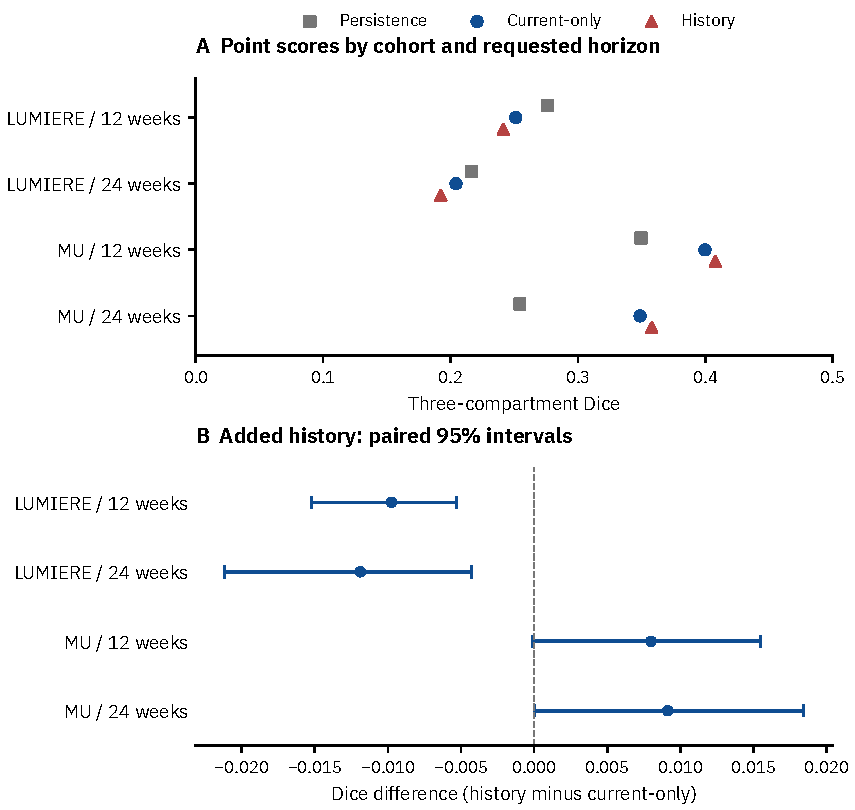
\includegraphics[width=\linewidth]{figures/updated_forecast.pdf}
\caption[Structured forecasts and added history]{Structured forecast Dice on reused selection patients. Higher is better. Panel A shows point scores for the weighted scenario-vote maps. Panel B shows history minus current-only with unadjusted 95\% paired patient-bootstrap intervals. LUMIERE has 112 targets/16 patients at 12 weeks and 89/15 at 24; MU has 36/18 and 22/13. Patients can contribute at both horizons.}\label{fig:structured}
\end{figure}
\FloatBarrier

History lowered Dice relative to current-only by 0.00975 on LUMIERE at 12 weeks and 0.01188 at 24 weeks, with both paired intervals below zero. MU differences were +0.00800 [-0.00010, +0.01551] and +0.00914 [+0.00004, +0.01844]. History had higher volume MAE in every cohort/horizon group. Its volume-CRPS contrasts with current-only and scalar-history controls all had intervals spanning zero.

The MU Dice gains over persistence were largely due to empty core compartments. At 24 weeks, current-only gained 9.44 percentage points overall; future-empty core contributed +10.26 points and nonempty core contributed -0.80 points under the original aggregate weights. Five of ten empty-core targets were correctly predicted empty. Three were resolutions from current reference volumes of 0.020, 0.045 and 0.662 mL; two were already empty. On the twelve targets whose core remained present, current-only Dice was 0.0422 below persistence, with a 95\% interval of [-0.0876, -0.0048].

Figure~\ref{fig:forecast-attribution} shows how the core strata and the other compartments contributed to the overall difference.
\begin{figure}[htbp]\centering
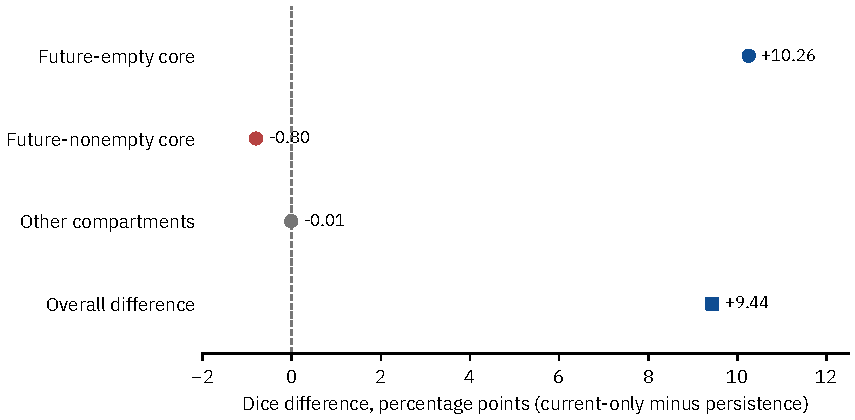
\includegraphics[width=\linewidth]{figures/updated_forecast_attribution.pdf}
\caption[Contributions to the MU 24-week forecast Dice difference]{Current-only minus model-persistence Dice on 22 MU 24-week targets from 13 reused selection patients. The first three points are contributions to the original patient-weighted, three-compartment aggregate, not within-group Dice differences. Other compartments combine compartments 1 and 3. The square is the overall difference. Values are in percentage points; points are descriptive estimates without intervals. Rounded contributions may not sum exactly to the rounded overall difference.}\label{fig:forecast-attribution}
\end{figure}

FLAIR abnormality showed a smaller gain across all 22 MU 24-week targets, each with a nonempty reference. Current-only improved Dice by 0.01264 [0.00414, 0.02144] over model persistence. Among 17 persistently nonempty targets from twelve patients whose reference volume changed by more than the larger of 2 mL or 20\% of its current value, the gain was 0.01456 [0.00547, 0.02439]. This supports a specific current-only gain in FLAIR-abnormality segmentation. It is a post-hoc development finding on 22 targets and requires independent confirmation.

Using the cavity-supervised observation state gives another current-only forecast comparison. At 24 weeks, original-three-compartment Dice increased from persistence's 0.2488 to 0.3760, while nonempty-core Dice fell from 0.1361 to 0.0123. Four-compartment volume CRPS improved from 16.4198 to 13.5597 mL; the scalar control scored 13.6599. Nonempty-core nominal 90\% coverage was 6.7\% at 12 weeks and 0\% at 24 weeks. The scalar control covered 93.3\% and 100\%, with wider intervals. The aggregate Dice gain therefore does not establish reliable recovery of nonempty core or calibrated uncertainty about its amount.

\section{Predicting compartment quantities}

The volume and coverage results motivate separating compartment presence and amount from spatial allocation. For the logistic quantity model, the 64-sample mean had 24-week nonempty-core MAE of 0.819 mL, compared with persistence at 1.281. Its exact fitted-distribution mean scored 1.769 mL. The corresponding Gaussian values were 1.475 and 1.691 mL. A small sample from these heavy-tailed distributions changed the apparent ranking. Deterministic CRPS was about 1.95--1.96 mL for both families at 24 weeks, against the frozen scalar control at 1.370.

Varying the fitting population and the available current and historical information gives 24 fits for comparison. The model receiving current MRI, history metadata, previous volumes and rates, and previous MRI had nonempty-core CRPS of 1.646 and 1.201 mL at 12 and 24 weeks, averaged across three seeds. Mean-volume MAE was 1.819 and 1.385 mL against persistence at 1.692 and 1.281. Nominal 90\% core coverage fell to 30.4\% and 25.0\%. No configuration met the required volume-error and CRPS conditions at both horizons under both the preselected seed and the average across three seeds.

Regularized scalar and PCA-MRI models use 156 fitting pairs from 56 patients and the same 58 selection targets. At 24 weeks, exact nonempty-core mean MAE was 11.065 mL for scalar inputs and 13.662 for added MRI components; CRPS was 2.571 and 2.686 mL. Both exceeded their persistence and scalar-distribution controls. Neither provides a satisfactory quantity model for spatial allocation: at each horizon, nonempty-core mean-volume MAE must be no worse than persistence and CRPS no worse than the scalar-distribution control. Neither model meets both conditions.

\section{Choosing MRI sequences}

The acquisition comparison tests whether predicted candidate features help choose the next sequence, using 48 MU visits from 16 development patients. Fixed, direct and JEPA policies chose the same path on every visit: T1, then CT1, then FLAIR. All score 0.62525 on anatomy utility averaged after observing two and three sequences. Identical choices leave no observed advantage for either learned policy. Oracle utility was 0.62709, a gain of 0.00184 [0.00010, 0.00410] under this observer and offline reveal task.

Missing-FLAIR completion improved against the preserved cavity-aware reference on every fixed input panel (Figure~\ref{fig:acquisition}). With T1, CT1 and T2 available, lesion MAE fell from 0.5879 to 0.5270. All four paired intervals favor the new observer, and every panel remains within the +0.05 retention allowance.

All-four-sequence anatomy Dice fell from 0.71769 to 0.67177, a difference of -0.04592 [-0.07020, -0.02220]. The interval crossed the -0.05 retention margin. Empty-core false-positive volume increased from 1.179 to 1.976 mL, and empty-cavity false positives increased from 4.516 to 8.908 mL. The observer improves completion while reducing anatomical agreement, so the gain depends on which readout is used. Its full four-sequence state occupies 16.09 GB; encoding averaged 12.84 seconds and the shared anatomy/image readout 1.58 seconds. These costs also limit its practicality as a patient state.

\FloatBarrier
\begin{figure}[htbp]\centering
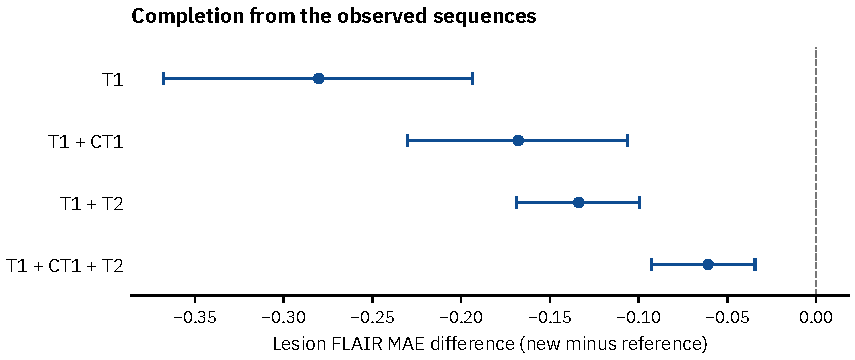
\includegraphics[width=\linewidth]{figures/updated_acquisition.pdf}
\caption[Missing-FLAIR completion in the acquisition study]{Lesion-region MAE differences in standardized intensity units on 48 MU visits from 16 development patients. Negative values favor the acquisition observer. Bars are paired 95\% patient-bootstrap intervals. The reference observer was trained on a broader population.}\label{fig:acquisition}
\end{figure}

\section{What predictive learning retains}

The preceding results judge representations through anatomical and image outputs. A clinical-classification comparison also tests whether the predictive objective adds useful information beyond direct adaptation, scoring ten patients. Calibrated log loss was 0.80850 for adapted direct BrainIAC, 0.81117 for proper JEPA and 0.81778 for shuffled-target JEPA; the fitting-prevalence control scored 0.70880. Proper JEPA was slightly worse than direct in both seeds. All declared objective contrasts had adjusted intervals spanning zero, providing no clear incremental benefit from the tested JEPA objective.

The shape-and-activity simulator makes the distinction between retained factors explicit. Predictive representations recover ellipse axes with normalized mean-squared error near 0.02, while the local activity factor remains poorly recovered, with a Brier score near 0.25. Direct factor supervision achieves activity Brier 0.10890 and 85.35\% accuracy. In this controlled setting, good recovery of global shape coexists with poor recovery of a local factor. A predictive objective alone does not ensure that a readout can recover every quantity needed for a downstream task.

\endgroup
